%%%%%%%%%%%%%%%%%%%%%%%%%%%%%%%%%%%%%%%%%
%
% Authors:
% Class by Felipe Portales-Oliva (f.portales.oliva@gmail.com) with template 
% content and modifications by Vel (vel@LaTeXTemplates.com)
%
% Enhanced by magicwenli 
%
%%%%%%%%%%%%%%%%%%%%%%%%%%%%%%%%%%%%%%%%%

\documentclass[
	12pt, % Default font size, values between 10pt-12pt are allowed
	%letterpaper, % Uncomment for US letter paper size
	cn, % Uncomment for Chinese
	%spanish, % Uncomment for Spanish
]{mwhw}

% Norm enhanced. Use \norm{}
\newcommand{\norm}[1]{\left\lVert#1\right\rVert}

% Template-specific packages
\usepackage[utf8]{inputenc} % Required for inputting international characters
\usepackage[T1]{fontenc} % Output font encoding for international characters

%----------------------------------------------------------------------------------------
%	ASSIGNMENT INFORMATION
%----------------------------------------------------------------------------------------

\title{Homework \#1} % Assignment title

\author{magicwenli} % Student name

\date{\today} % Due date

\institute{Xi'an Jiao Tong University \\ Computer Science and Technology} % Institute or school name

\class{异世界生活技巧} % Uncomment for Course or class name

\professor{Mr. WenLi} % Uncomment for Professor or teacher in charge of the assignment

\IDnumber{APTX4396} % Uncomment for ID in charge of the assignment

\classID{中土大陆一班} % Uncomment for classID in charge of the assignment

%----------------------------------------------------------------------------------------

\begin{document}

\maketitle % Output the assignment title, created automatically using the information in the custom commands above

%----------------------------------------------------------------------------------------
%	ASSIGNMENT CONTENT
%----------------------------------------------------------------------------------------

\section*{问题框}

\begin{problem}
	证明:范数$\norm{\cdot}$的对偶范数满足范数的定义
	\begin{equation*}
	    \norm{z}_*=sup\{z^Tx:\ \norm{x}\leq1\}=sup\{z^Tx:\ \norm{x}=1\}
	\end{equation*}
\end{problem}


%------------------------------------------------

\subsection*{回答}
    \begin{equation*}
        \norm{z}_*=\max_{\norm{x}\leq 1}\sum{z_ix_i}
    \end{equation*}
    \begin{enumerate}
    \item 正定性:
    如果$z=0$,显然$\norm{0}_*=0$.
    \item 非负性:
    如果$z\neq 0$,则$\norm{x}\neq 0$. 由于$x=\frac{z}{\norm{z}}$,有$\norm{z}_*\leq \frac{\norm{z}^2_2}{\norm{z}}>0$.\\
    特别的,如果$\norm{z}_*=0$,则必有$z=0$.
    \item 齐次性:\\
    由范数定义,有:
    \begin{equation*}
        \norm{tz}_*=\max_{\norm{x}\leq 1} | z^Ttx|=\max_{\norm{x}\leq 1}|t||z^Tx |=|t| \max_{\norm{x}\leq 1} | z^Tx |=|t|\norm{z}_*
    \end{equation*}
\end{enumerate}

%----------------------------------------------------------------------------------------
\section*{插入浮动体}
\begin{figure}[htb]
	\centering
	\includegraphics[width=16cm]{src/shuDian-313}
	%\caption{电路图}
\end{figure}
%------------------------------------------------
\subsection*{插入tikz流程图}
\begin{enumerate}
	\item Mealy型:
	\begin{center}
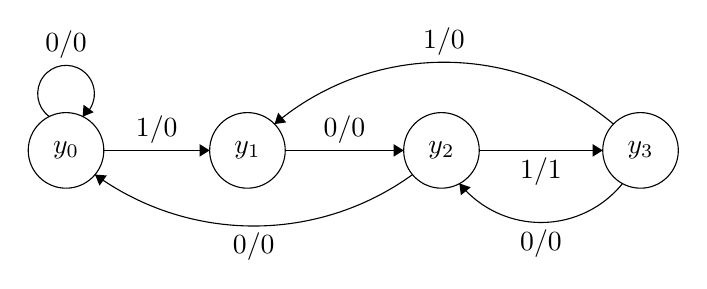
\begin{tikzpicture}[scale=0.16]
\tikzstyle{every node}+=[inner sep=0pt]
\draw [black] (10,-26.7) circle (3);
\draw (10,-26.7) node {$y_0$};
\draw [black] (24.4,-26.7) circle (3);
\draw (24.4,-26.7) node {$y_1$};
\draw [black] (39.8,-26.7) circle (3);
\draw (39.8,-26.7) node {$y_2$};
\draw [black] (55.6,-26.7) circle (3);
\draw (55.6,-26.7) node {$y_3$};
\draw [black] (13,-26.7) -- (21.4,-26.7);
\fill [black] (21.4,-26.7) -- (20.6,-26.2) -- (20.6,-27.2);
\draw (17.2,-26.2) node [above] {$1/0$};
\draw [black] (27.4,-26.7) -- (36.8,-26.7);
\fill [black] (36.8,-26.7) -- (36,-26.2) -- (36,-27.2);
\draw (32.1,-26.2) node [above] {$0/0$};
\draw [black] (42.8,-26.7) -- (52.6,-26.7);
\fill [black] (52.6,-26.7) -- (51.8,-26.2) -- (51.8,-27.2);
\draw (47.7,-27.2) node [below] {$1/1$};
\draw [black] (26.548,-24.61) arc (130.09656:49.90344:20.885);
\fill [black] (26.55,-24.61) -- (27.48,-24.48) -- (26.84,-23.71);
\draw (40,-19.2) node [above] {$1/0$};
\draw [black] (8.677,-24.02) arc (234:-54:2.25);
\draw (10,-19.45) node [above] {$0/0$};
\fill [black] (11.32,-24.02) -- (12.2,-23.67) -- (11.39,-23.08);
\draw [black] (37.5,-28.622) arc (-54.11064:-125.88936:21.494);
\fill [black] (12.3,-28.62) -- (12.66,-29.5) -- (13.24,-28.69);
\draw (24.9,-33.2) node [below] {$0/0$};
\draw [black] (54.176,-29.322) arc (-38.84397:-141.15603:8.315);
\fill [black] (41.22,-29.32) -- (41.34,-30.26) -- (42.12,-29.63);
\draw (47.7,-32.92) node [below] {$0/0$};
\end{tikzpicture}
\end{center}
Moore型:
\begin{center}
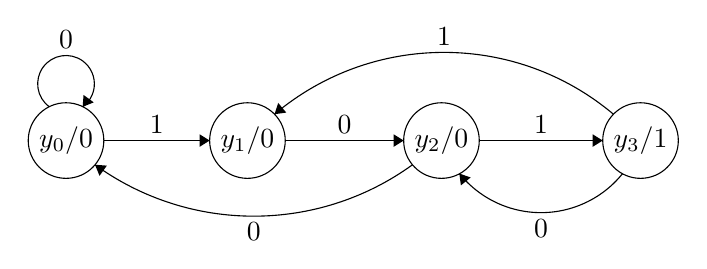
\begin{tikzpicture}[scale=0.16]
\tikzstyle{every node}+=[inner sep=0pt]
\draw [black] (10,-26.7) circle (3);
\draw (10,-26.7) node {$y_0/0$};
\draw [black] (24.4,-26.7) circle (3);
\draw (24.4,-26.7) node {$y_1/0$};
\draw [black] (39.8,-26.7) circle (3);
\draw (39.8,-26.7) node {$y_2/0$};
\draw [black] (55.6,-26.7) circle (3);
\draw (55.6,-26.7) node {$y_3/1$};
\draw [black] (13,-26.7) -- (21.4,-26.7);
\fill [black] (21.4,-26.7) -- (20.6,-26.2) -- (20.6,-27.2);
\draw (17.2,-26.2) node [above] {$1$};
\draw [black] (27.4,-26.7) -- (36.8,-26.7);
\fill [black] (36.8,-26.7) -- (36,-26.2) -- (36,-27.2);
\draw (32.1,-26.2) node [above] {$0$};
\draw [black] (42.8,-26.7) -- (52.6,-26.7);
\fill [black] (52.6,-26.7) -- (51.8,-26.2) -- (51.8,-27.2);
\draw (47.7,-26.2) node [above] {$1$};
\draw [black] (26.548,-24.61) arc (130.09656:49.90344:20.885);
\fill [black] (26.55,-24.61) -- (27.48,-24.48) -- (26.84,-23.71);
\draw (40,-19.2) node [above] {$1$};
\draw [black] (8.677,-24.02) arc (234:-54:2.25);
\draw (10,-19.45) node [above] {$0$};
\fill [black] (11.32,-24.02) -- (12.2,-23.67) -- (11.39,-23.08);
\draw [black] (37.5,-28.622) arc (-54.11064:-125.88936:21.494);
\fill [black] (12.3,-28.62) -- (12.66,-29.5) -- (13.24,-28.69);
\draw (24.9,-33.2) node [below] {$0$};
\draw [black] (54.176,-29.322) arc (-38.84397:-141.15603:8.315);
\fill [black] (41.22,-29.32) -- (41.34,-30.26) -- (42.12,-29.63);
\draw (47.7,-32.92) node [below] {$0$};
\end{tikzpicture}
\end{center}
\item Mealy型:
\begin{center}
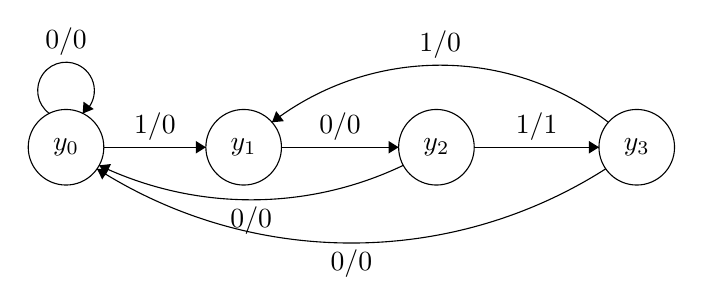
\begin{tikzpicture}[scale=0.16]
\tikzstyle{every node}+=[inner sep=0pt]
\draw [black] (10.3,-26.7) circle (3);
\draw (10.3,-26.7) node {$y_0$};
\draw [black] (24.4,-26.7) circle (3);
\draw (24.4,-26.7) node {$y_1$};
\draw [black] (39.7,-26.7) circle (3);
\draw (39.7,-26.7) node {$y_2$};
\draw [black] (55.6,-26.7) circle (3);
\draw (55.6,-26.7) node {$y_3$};
\draw [black] (13.3,-26.7) -- (21.4,-26.7);
\fill [black] (21.4,-26.7) -- (20.6,-26.2) -- (20.6,-27.2);
\draw (17.35,-26.2) node [above] {$1/0$};
\draw [black] (27.4,-26.7) -- (36.7,-26.7);
\fill [black] (36.7,-26.7) -- (35.9,-26.2) -- (35.9,-27.2);
\draw (32.05,-26.2) node [above] {$0/0$};
\draw [black] (42.7,-26.7) -- (52.6,-26.7);
\fill [black] (52.6,-26.7) -- (51.8,-26.2) -- (51.8,-27.2);
\draw (47.65,-26.2) node [above] {$1/1$};
\draw [black] (8.977,-24.02) arc (234:-54:2.25);
\draw (10.3,-19.45) node [above] {$0/0$};
\fill [black] (11.62,-24.02) -- (12.5,-23.67) -- (11.69,-23.08);
\draw [black] (37.068,-28.137) arc (-64.44698:-115.55302:27.977);
\fill [black] (12.93,-28.14) -- (13.44,-28.93) -- (13.87,-28.03);
\draw (25,-31.37) node [below] {$0/0$};
\draw [black] (26.648,-24.717) arc (127.49495:52.50505:21.935);
\fill [black] (26.65,-24.72) -- (27.59,-24.63) -- (26.98,-23.83);
\draw (40,-19.69) node [above] {$1/0$};
\draw [black] (53.138,-28.413) arc (-57.469:-122.531:37.541);
\fill [black] (12.76,-28.41) -- (13.17,-29.26) -- (13.71,-28.42);
\draw (32.95,-34.8) node [below] {$0/0$};
\end{tikzpicture}
\end{center}
Moore型:
\begin{center}
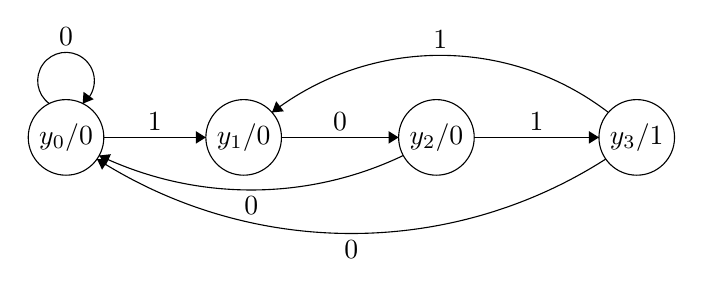
\begin{tikzpicture}[scale=0.16]
\tikzstyle{every node}+=[inner sep=0pt]
\draw [black] (10.3,-26.7) circle (3);
\draw (10.3,-26.7) node {$y_0/0$};
\draw [black] (24.4,-26.7) circle (3);
\draw (24.4,-26.7) node {$y_1/0$};
\draw [black] (39.7,-26.7) circle (3);
\draw (39.7,-26.7) node {$y_2/0$};
\draw [black] (55.6,-26.7) circle (3);
\draw (55.6,-26.7) node {$y_3/1$};
\draw [black] (13.3,-26.7) -- (21.4,-26.7);
\fill [black] (21.4,-26.7) -- (20.6,-26.2) -- (20.6,-27.2);
\draw (17.35,-26.2) node [above] {$1$};
\draw [black] (27.4,-26.7) -- (36.7,-26.7);
\fill [black] (36.7,-26.7) -- (35.9,-26.2) -- (35.9,-27.2);
\draw (32.05,-26.2) node [above] {$0$};
\draw [black] (42.7,-26.7) -- (52.6,-26.7);
\fill [black] (52.6,-26.7) -- (51.8,-26.2) -- (51.8,-27.2);
\draw (47.65,-26.2) node [above] {$1$};
\draw [black] (8.977,-24.02) arc (234:-54:2.25);
\draw (10.3,-19.45) node [above] {$0$};
\fill [black] (11.62,-24.02) -- (12.5,-23.67) -- (11.69,-23.08);
\draw [black] (37.068,-28.137) arc (-64.44698:-115.55302:27.977);
\fill [black] (12.93,-28.14) -- (13.44,-28.93) -- (13.87,-28.03);
\draw (25,-31.37) node [below] {$0$};
\draw [black] (26.648,-24.717) arc (127.49495:52.50505:21.935);
\fill [black] (26.65,-24.72) -- (27.59,-24.63) -- (26.98,-23.83);
\draw (40,-19.69) node [above] {$1$};
\draw [black] (53.141,-28.417) arc (-57.36292:-122.63708:37.439);
\fill [black] (12.76,-28.42) -- (13.16,-29.27) -- (13.7,-28.43);
\draw (32.95,-34.83) node [below] {$0$};
\end{tikzpicture}
\end{center}
\end{enumerate}
%----------------------------------------------------------------------------------------
\newpage
\section*{插入跨页长表}
该状态表中有$9$个状态,应选取$4$个状态变量$y_0y_1y_2y_3$,即状态变量数$K=3$,输入组合数$p=2$,输出函数位数$q=1$.
\begin{longtable}[c]{@{}ccccc@{}}
\toprule
状态 & 规则I(R) & 规则II(m) & 规则III(l) & 总改善效果(E) \\* \midrule
\endhead
%
\bottomrule
\endfoot
%
\endlastfoot
%
Q0Q1 & 1 & 1 & 0 & 5 \\
Q0Q2 & 1 & 1 & 0 & 5 \\
Q0Q3 & 1 & 0 & 0 & 3 \\
Q0Q4 & 1 & 1 & 0 & 5 \\
Q0Q5 & 0 & 1 & 0 & 2 \\
Q0Q6 & 1 & 1 & 0 & 5 \\
Q0Q7 & 1 & 1 & 0 & 5 \\
Q0Q8 & 0 & 1 & 0 & 2 \\
Q1Q2 & 0 & 0 & 1 & 1 \\
Q1Q3 & 1 & 1 & 1 & 6 \\
Q1Q4 & 1 & 0 & 1 & 4 \\
Q1Q5 & 0 & 0 & 1 & 1 \\
Q1Q6 & 1 & 1 & 1 & 6 \\
Q1Q7 & 1 & 0 & 1 & 4 \\
Q1Q8 & 0 & 0 & 1 & 1 \\
Q2Q3 & 0 & 0 & 1 & 1 \\
Q2Q4 & 0 & 0 & 1 & 1 \\
Q2Q5 & 0 & 0 & 1 & 1 \\
Q2Q6 & 0 & 0 & 1 & 1 \\
Q2Q7 & 0 & 0 & 1 & 1 \\
Q2Q8 & 0 & 0 & 1 & 1 \\
Q3Q4 & 1 & 0 & 1 & 4 \\
Q3Q5 & 0 & 0 & 1 & 1 \\
Q3Q6 & 1 & 0 & 1 & 4 \\
Q3Q7 & 1 & 0 & 1 & 4 \\
Q3Q8 & 0 & 0 & 1 & 1 \\
Q4Q5 & 0 & 0 & 1 & 1 \\
Q4Q6 & 1 & 0 & 1 & 4 \\
Q4Q7 & 1 & 0 & 1 & 4 \\
Q4Q8 & 0 & 0 & 1 & 1 \\
Q5Q6 & 0 & 0 & 1 & 1 \\
Q5Q7 & 0 & 0 & 1 & 1 \\
Q5Q8 & 0 & 0 & 1 & 1 \\
Q6Q7 & 1 & 0 & 1 & 4 \\
Q6Q8 & 0 & 0 & 1 & 1 \\
Q7Q8 & 0 & 0 & 1 & 1 \\* \bottomrule
\caption{规则满足情况}
\label{tab:3}\\
\end{longtable}

\section{代码}
\begin{lstlisting}
#include <stdio.h>
#include <pthread.h>

int value=0;
void *runner(void *param); /* the thread */
int main()
{
   int pid;
   pthread_t tid;
   pthread_attr_t attr;
   pid=fork();
   if(pid==0)
   {
      pthread_attr_init(&attr);
      pthread_create(&tid, &attr, runner, NULL);
      pthread_join(tid, NULL);
      printf("CHILD: value=%d\n", value);  /* LINE C */
   }else if(pid>0){
      wait(NULL);
      printf("PARENT: value=%d\n",value); /* LINE P */
   }
}
void *runner(void *param)
{
   value=5;
   pthread_exit(0);
}
\end{lstlisting}

\end{document}


% \begin{center}
% 	\includegraphics[width=0.5\columnwidth]{swallow.jpg} % Example image
% \end{center}
